\chapter{Implementation}
\chlab{implementation}

A system for fragment-based molecule parameterisation has three distinct tasks: visualising a molecule, finding matching fragments for that molecule, and allowing for interaction with the molecule and its matching fragments. As these tasks can be performed in isolation, it has been decided to implement the molecule parameterisation tool as three separate systems.

The front-end of the system, where users will carry out the parameterisation process, will be called the Online tool for Fragment-based Molecule Parameterisation~(\oframp). This name will also be used to refer to the system as a whole, as it is the hart of the system and is dependent on the other systems. The molecule is also visualised in \oframp, but the for this purpose essential, calculations of atom positions are done in the Online tool for Atom Position Calculations~(\oapoc). Finally, finding matching fragments and sorting them based on relevance is done by the Online tool for Molecule Fragment Finding~(\omfraf).

The complete network diagram for the fragment-based molecule parameterisation system is shown in \figref{diagram}. It is clear that \oframp{} is the central system, but that the more computation-intensive tasks are carried out by \oapoc{} and \omfraf{}. The remainder of this chapter will discuss each of the systems in more detail.


\begin{sidewaysfigure}[p]
\begin{center}
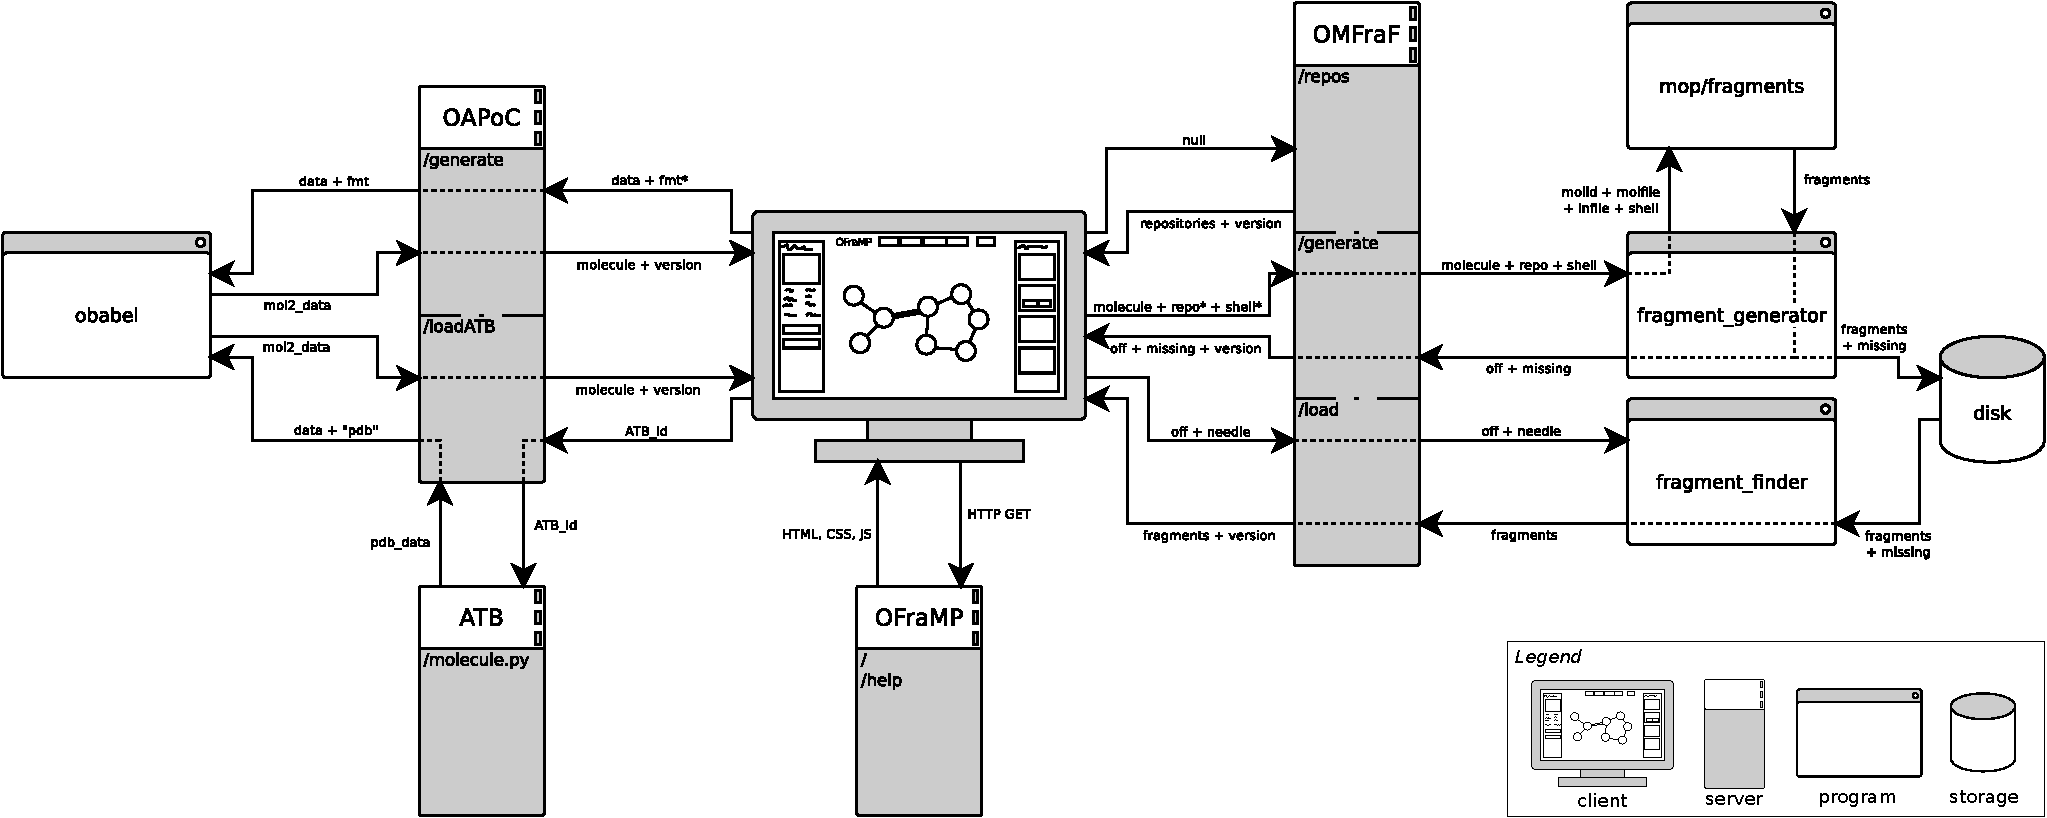
\includegraphics[width=\textwidth]{img/network_diagram.pdf}
\vspace{1em}
\caption{Network diagram of \oframp and its supporting systems.}
\figlab{diagram}
\end{center}
\end{sidewaysfigure}


\section[\oframp]{The Online tool for Fragment-based Molecule Parameterisation}
\oframp{} is the central part of the fragment-based molecule parameterisation system. It contains the user interface and connects with \oapoc{} and \omfraf{}. As discussed in \secref{platform}, it has been decided to implement the system as a web application. Following the current trend in web applications, \oframp{} has been implemented using the latest techniques from \verb|HTML5|, \verb|CSS3| and \verb|JavaScript|.

Using the latest web technologies allows for great cross-platform support. It allows the system to run on any desktop and laptop operating system, and creates the possibility of running it on a smartphone or tablet\footnote{This has not been a requirement for the project and has therefore not been tested extensively}, although the limited size of a smartphone screen can be problematic. Using the latest \verb|HTML5| technologies, however, also comes at a cost. Older browsers generally lack support, and will therefore not be able to run \oframp. Luckily, according to the latest browser statistics from StatCounter~\cite{statcounter2014statcounter}, almost 85\% of internet users uses a browser that has full support for these technologies. Thanks to the Internet Explorer canvas fallback \verb|excanvas|~\cite{arvidsson2009explorercanvas}, partial support can be provided for an additional 11\% of people, which results in a total support for 96\% of internet users.

\nlipsum

\begin{figure}[h!]
\begin{center}
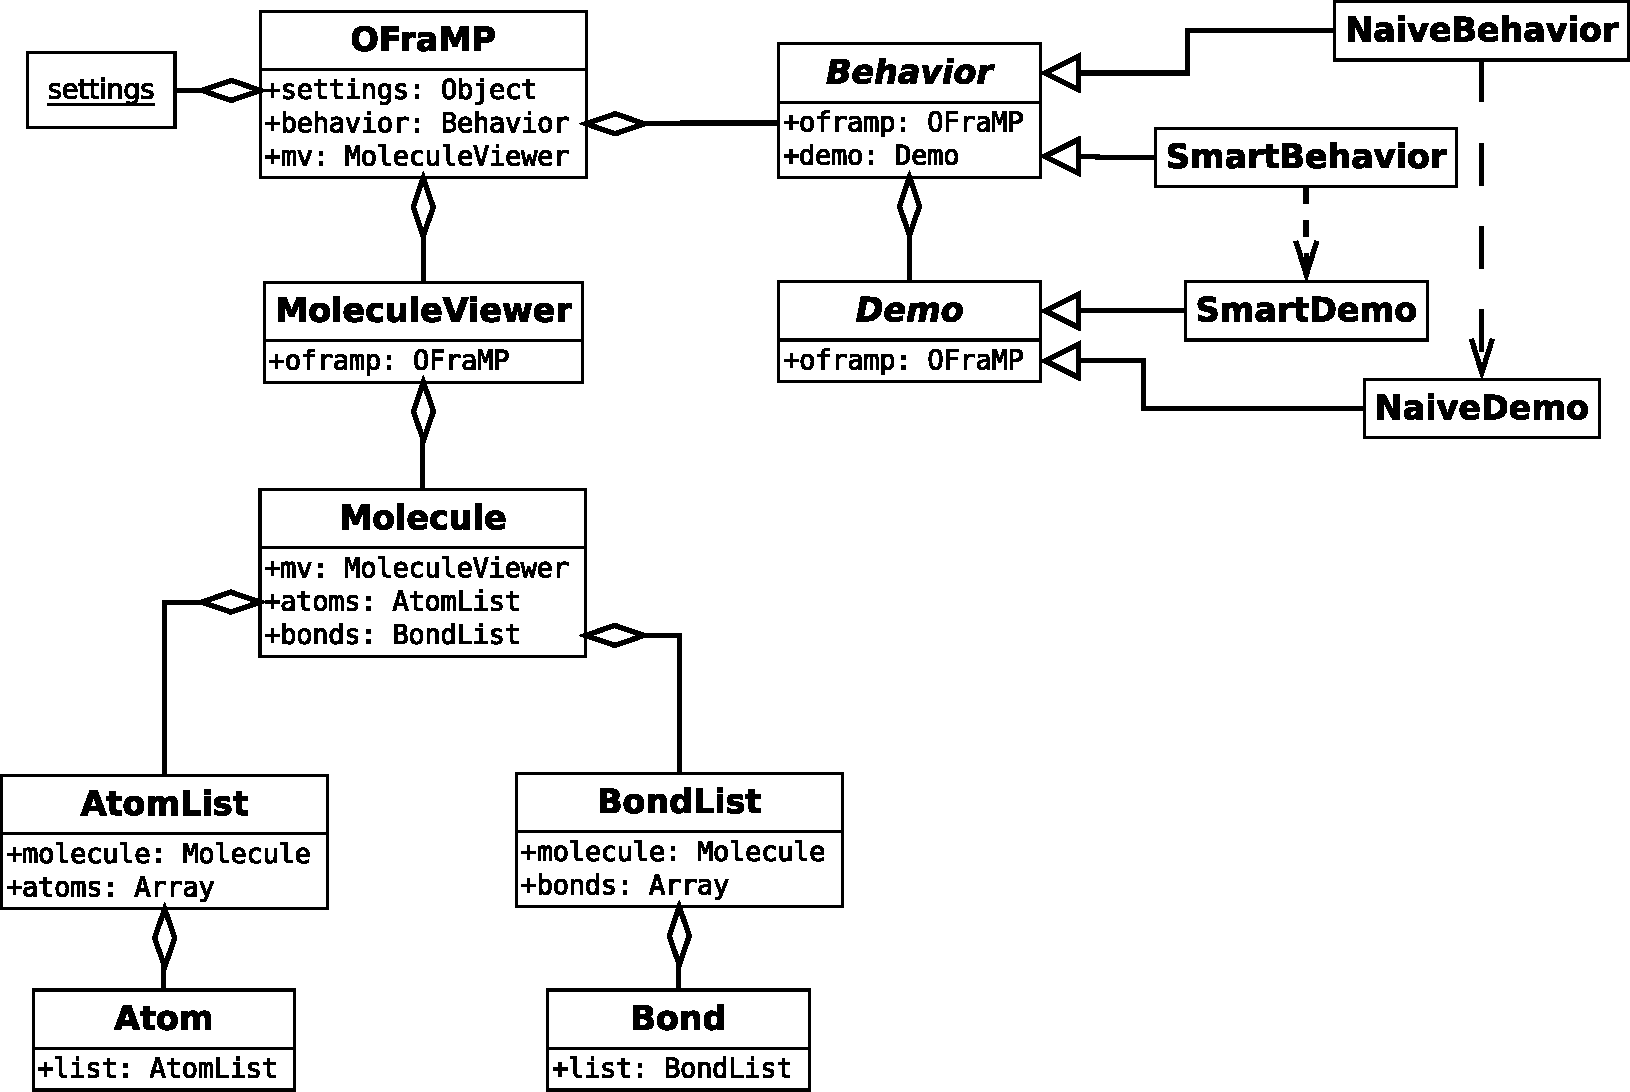
\includegraphics[width=\textwidth]{img/oframp_class.pdf}
\caption{Simplified class diagram of \oframp.}
\figlab{oframp_class}
\end{center}
\end{figure}

\subsection{Visualisation}
\nlipsum

\subsection{Interaction}
We use LGF files~\cite{dezso2011lemon}\ldots

\nlipsum


\section[\oapoc]{The Online tool for Atom Position Calculations}
\nlipsum

\subsection{obabel}
\nlipsum


\section[\omfraf]{The Online tool for Molecule Fragment Finding}
\nlipsum

\subsection{Generation}
\nlipsum

\subsubsection{mop/fragments}
\nlipsum

\subsection{Finding}
\nlipsum
